\chapter{Introduction}
\section{Motivation}
%Robot => speech => MIDI (history)
From the machnical music performing antomata, to the Japanese virtual signer Hatune Miku, there had been many attempts to create autoated system that performs music. However, many of these system can only perform predefined expression, which is not very satisfying. State-of-the-art text-to-speech system can already generate fluid and natural speech, but computer performance still can't perform very expressivly.

Therefore, many researcher have devoted many effort to develop systems that can automatically or semi-automatically perform music expressively. There is even a biannual contest called Music Performance Rendering Contest (RenCon)\cite{rencon} that puts all performance system to into competition. Their roadmap suggest that they wish to win the Chopin International Piano Contest by a computer perforer. We will review previous works, including many which won the RenCon prizes, in Chapter \ref{chap:prev}.
%Computer generated music, such as synthsized MIDI, are often considered robotic and unexpressive. But we have already witnessed the fluid and lively sound generated by state-of-the-art text-to-speech systems. This inspired us to develop a system that can read a music score and play it in an expressive, humanly way. Such system can be used for audiolizing score notation editing software, creating interactive media content, and generating royality-free music. 

%Established pianists always has his/her own distinctive style. Such sytle distinguised himself/herself from all the other pianists. If the expressive performance system can learn the style of a performer, it might be able to provide musicological insight of performance styles. Furthermore, we can even make a mastero who is no longer with us play music he/she never played in his/her lifetime.

There are many applications for a computer expressive performance system, many commercial music typesetting software like Finale and Sibelius already have expressive playback features built-in. On the commercial side, such system can provide personalized music listening experience. For the music production industry, it saved a lot of cost on hiring musicians or licensing. Such system can also opens up new opportunity in music making, such as human-machine co-performance, or interactive multimedia installation. In academia, researchers can use this technology to model the performing style of musicians, or restore historical music archive.

\framebox{TODO:Discuss Mazolla's theroy of expressive performance}

%\begin{figure}[tp]
%   \begin{center}
%      %TODO:Fig.: expressive performance concept
%      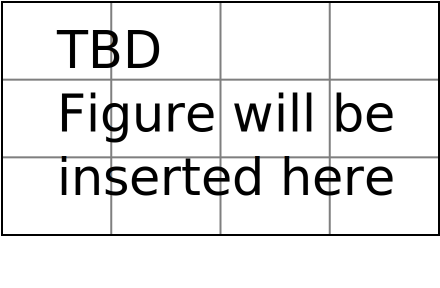
\includegraphics[width=\textwidth]{fig/TBDFigure}
%
%   \end{center}
%   \caption{From Composer to Performance}
%   \label{fig:concept}
%\end{figure}
%Application: musicology study, typesetting tool, play score archive, play computer-generated music, accompaniment



\section{Goal and Contribution}
\framebox{TODO:brief guide to previous works}
There are many different goals for computer expressive performance, which will be discussed in Chapter \ref{chap:prev}. In this research the ultimate goal is to be able to play any music in any expressive style specified. But due to the technical and time constrain, we need to set a more practical goal for our research. We wish to build a computer expressive performance system based on an offline supervised learning algorithm. The system will be able to learn any play monophonic musical phrases. The expressiveness will be at phrase level, structural or timbre related expression are not the primary concern. The performance style will be controlled by the learning material, which is traditional music notation, with human-annotated phrasing information. If only recordings from a single performer is given, it should learn the particular style of the performer.


The major contribution of this thesis is that we apply structural support vector machine on expressive performance problem. There exist no previous work that uses the discriminative learning power of support vector machine on computer expressive performance question. We also developed methods and tools to generate corpus for expressive performance system based on learning algorithms. 
%\bibliographystyle{unsrt}
%\bibliography{thesisbib}
\section{Chapter Organization}
In Chapter \ref{chap:prev}, we will give an overview of previous works and their varying goals, the works will be grouped by the way they learn performance knowledge, and finally we will discuss some additional specialities such as special instrument model or special user interaction pattern. In Chapter \ref{chap:proposed}, we will first give a brief introduction to the mathematical background of the learning algorithm, SVM-HMM. And then we will provide a top-down explanation to the proposed method. Then in Chapter \ref{chap:corpus}, we will explain how the corpus used for training is designed and implemented. Finally, In Chapter \ref{chap:exp}, we will show several experiment results and discussions. We have also included two appendixes, appendix \ref{chap:sw} presents some software tools used in this research, which may be helpful for other researchers in music and machine learning fields.
